\documentclass[12pt]{article}
\usepackage[utf8]{inputenc}
% \usepackage[english, russian]{babel}
\usepackage[colorlinks=true,urlcolor=darkgray,citecolor=darkgray,linkcolor=darkgray,bookmarks=true]{hyperref}
% \usepackage{ccaption}
\usepackage{authblk}
\usepackage{indentfirst}
% \usepackage{float} 
\usepackage{amsmath}
% \usepackage{apacite}
\usepackage{natbib}
\usepackage{graphicx}
\usepackage{comment}
\usepackage{amsfonts}
\usepackage{bm}
\usepackage{amssymb}
\usepackage{amsthm}
\usepackage{mathtools}
\usepackage{upgreek} % AMS
\usepackage{marvosym}
\usepackage{threeparttable}
\usepackage{etoolbox}
\usepackage{cmap}	
\usepackage[nospace]{varioref}	
\usepackage{cleveref}
\usepackage{multirow}
\usepackage{fullpage} 
\usepackage{geometry}
\geometry{
 a4paper,
 total={210mm,297mm},
 left=20mm,
 right=20mm,
 top=20mm,
 bottom=20mm,
 }
\usepackage{url}
\usepackage{pgfplots}
\usepackage{caption}
\usepackage{longtable}
\usepackage{multirow}
\usepackage{booktabs}
\usepackage{pgf}
\usepackage{tikz}
\pgfplotsset{compat=1.15}
\usepackage{mathrsfs}
\usepackage{tikz} 
\usepackage{pgfplots}
\usepackage{pgfplotstable}
\usepackage{braket}
% \usepackage[capposition=top]{floatrow}
\usepackage{verbatim}
% \usepackage[position=bottom]{subfig}
\usepackage{graphicx}
%\usefonttheme[onlymath]{serif}
\usepackage[colorinlistoftodos]{todonotes}
\usepackage{setspace}
\usetikzlibrary{arrows}
\usetikzlibrary{calc}
\usetikzlibrary{positioning}
\usetikzlibrary{fit}
\usetikzlibrary{backgrounds}
\usetikzlibrary{intersections}
\tikzset{
style1/.style={
line cap=round,line join=round,
axis/.style={thick, ->, >=stealth'},
l/.style={thin},
d/.style={dashed, thin}, 
pile/.style={thin, <->, >=stealth',shorten <=3pt, shorten >=3pt}, 
every node/.style={color=black}, 
}
}




% \usepackage[backend=biber,
% style=chicago-authordate]{biblatex}
% \addbibresource{references.bib}

\def\references{
    \bibliography{misc/references.bib}
    \bibliographystyle{misc/econ}
}



\usepackage{parskip}

\setlength{\parindent}{15pt}
\onehalfspacing

    \makeatletter 

% \renewcommand{\maketitle}{\begin{center}
%         \noindent{\bfseries\scshape\Large\@title} 
%         \noindent{ \itshape\large\card{\subtitle}} 
%         \par  \vspace{0.5ex}
%         \noindent {\large\itshape\@author}
%         \noindent{\card{\footnotesize \itshape \extratext}}
%         \end{center}
%         } 

    % \makeatother
    % \def\extratext{}
    % \def\topic{}
    % \def\subtitle{}
       
 \newcommand{\card}[1]{ \ifthenelse{\equal{#1}{}}{}{ {\par#1}}}

 \usepackage{lipsum}

 \makeatletter
 \def\blfootnote{\gdef\@thefnmark{$\dagger$}\@footnotetext}
 \makeatother




    %%% Работа с картинками
    \usepackage{graphicx}  % Для вставки рисунков
    \setlength\fboxsep{3pt} % Отступ рамки \fbox{} от рисунка
    \setlength\fboxrule{1pt} % Толщина линий рамки \fbox{}
    \usepackage{wrapfig} % Обтекание рисунков текстом
    \usepackage{rotating}%поворот figure


    \DeclareRobustCommand{\firstsecond}[2]{#1}


    \makeatletter
\newcommand\footnoteref[1]{\protected@xdef\@thefnmark{\ref{#1}}\@footnotemark}
\makeatother


\usepackage{rotating}
% \usepackage{caption}
\usepackage{subcaption}
\captionsetup{labelfont=bf, labelsep=period, skip=0pt}


\graphicspath{{./../Figures}}


\usepackage{makecell}
\usepackage{dcolumn}

\title{Verifying HANK.\\ Evidence from size-persistence tradeoff}
\author{Alexander I. Vlasov\thanks{Email: avlasov(at)nes.ru. For supplementary materials, such as replication code and datasets, see the repository \href{https://rb.gy/jzhch9}{rb.gy/jzhch9}.}}
\date{\normalsize First version: January, 2024\\\vspace{1ex} This version: January, 2024\\ \vspace{1ex}
\href{https://github.com/alvlsv/CheckingHank/blob/6906f23fcb1a16aa4fc9997532f52c1659e9c29f/Checking_HANK/Paper/CheckingHANK.pdf}{Click here for the most recent draft}}
\numberwithin{equation}{section}
\begin{document}

% \maketitlenew
\selectlanguage{english}
\maketitle



\begin{abstract}
    \noindent This work explores size-persistence tradeoff for monetary policy in the manner most close to its original formulation by Kaplan, Moll, and Violante (2018). 
    \\
    \noindent\textbf{Keywords:} Monetary Policy, Heterogeneous Agents, New Keynesian, Consumption
    \\
    \noindent\textbf{JEL Codes:} E21, E52, E12 \\
    \bigskip
\end{abstract}

\section{Introduction}

The prerequisite for the successful conduction of monetary response to a shock is the good understanding of Monetary Transmission Mechanism (MTM) -- the way that external changes in short term rate translate into the economy. 
Traditionally, macroeconomic models assumed away all of the heterogeneity in agents, replacing each with a representative one \cite{Gali2018}.
This representative agent models\footnote{Further referred to under abbreviated name RANK, what stands for Representative Agent New Keynesian (model).} are distinguished by the fact that they show the economy in a much more compact and tractable manner than heterogeneous ones.
Although, assumption of insignificance of differences between households looks quite unrealistic, it is still not immediately obvious, whether heterogeneity in a particular agent traits actually enhances the predictive powers of Representative-Agent New Keynesian (RANK) models\footnote{For example, \citet{Krusell1998} argue that  ``the behavior of the macroeconomic aggregates can be almost perfectly described using only the mean of the wealth distribution''.} 
and whether this result would hold to the data.

This paper conduct an econometric check of one of distinct outcomes of Heterogeneous-Agent New Keynesian (HANK) model by \citet[henceforth, KMV]{KMV2018}, namely size-persistence tradeoff. 


One of the most important problem in RANK is that, in equilibrium all of the agents are neither savers nor borrowers, even in the absence of financial frictions \cite{Gali2018}. 
This happens because every agent in the model is identical, and therefore, the only possible channel through which monetary policy could work, in theory, is the intertemporal substitution channel.
But this this questioned by the fact that aggregated time-series data on consumption finds a small sensitivity of consumption to changes in the interest rate after controlling for income changes \cite{Campbell1989, Canzoneri2007} -- ``imperfect consumption insurance''. 
Although by itself, it cannot be concluded from this evidence that the effect of intertemporal substitution is small, because indirect effects can almost completely compensate for changes caused by substitution.


\citet{KMV2018} served as a way to answer the accumulated questions about modeling the economy in a neo-Keynesian manner. 
The key idea is that some of the households face financial frictions i.e borrowing limit, which make them more sensitive to income change and less sensitive to shock of interest rate, since household cannot smooth the unexpected temporal income shock with the increase in credit.


\subsection{Trade-offs in HANK}

HANK, since it was not reversely-engineered, requires not only a ``check for inputs''\footnote{The Hand-to-Mouth household existence, which was done in  \citet{KVW2014}, and in \citet{Cloyne2019}.} but also a ``check for outputs'' -- the monetary policy outcomes.
HANK, as formulated by KMV has two main monetary policy tradeoffs:
tradeoff between size and persistence of monetary shock, and inflation-activity tradeoff.
In this work we focus on the former tradeoff.
It could be summarized as following: the higher the autocorrelation of monetary shock, the lower the elasticity of consumption to the expected path deviation of the rate of interest from its natural value.\footnote{Further we sometimes  refer to a difference between real rate and neutral (natural) rates of interest as the excess rate}
Intuitively, persistence of highly autocorrelated shock is indifferent to non-HtMs, as it is in RANK, since the only channel of monetary transmission is intertemporal substitution, but it matters for HtM households, whose response may be dampened by the persistence of monetary shock. 
This effect stems from failure of Ricaridan equivalence, since when it fails, then ``not only timing of fiscal policy but timing of monetary policy matters as well'' \cite{KMV2018}.





\subsection{Related literature}


First, this work provides additional indirect empirical support for models focused on the role of heterogeneity in household portfolio in MTM, for example \citet{KMV2018}, \citet{Auclert2019}, \citet{Luetticke2021} and successors.
There were several studies, which empirically support HANK. 

Most of the literature exploring the empirical side of HANK uses the individual level portfolio data. \citet{HolmPaulTischbirek2020} explores the norwegian individual-level dataset in trying to investigate the full process of the transmission of monetary policy.
They find that the low-liquidity households (\citeauthor{KMV2018} would call them hand-to-mouth households) show strong responce to monetary shock estimated with \cite{RomerRomer2004} identification strategy.
Another work lying in the same field is \citet{Cloyne2019}, which  shows that aggregate response of consumption to interest rate is mostly driven by households with a mortgage -- balance sheet driven heterogeneity plays a key role in monetary policy transmission.
It finds, that, in response to a negative monetary shock, the expenditure rise is highly significant for mortgagors\footnote{As \citet{Cloyne2019} shows, mortgagors and Wealthy HtMs as defined by \citet{KVW2014} are extremely overlapping groups.}, less significant for renters, and insignificant for owners with controls for different characteristics.
Another empirical contribution to of literature is done by \citet{Gross2020}, they document the MPC change over economic cycle, specifically its change through GFC.

%add


This work contribute to the discussion with conformation of the size-persistence tradeoff existence, and confirmation that it has a quadratic form.
Since this trade-off is the first of two KMV HANK's outcomes, this work gives us additional confidence to believe in the validity of this model essentials -- the importance and significance of indirect effects of monetary policy on consumption.
At the same time this work does focus on the overall effect, not trying to disentangle the direct and different indirect channels\footnote{which could give additional multiplicative effect of the monetary policy shock}, since the total effect is what actually we need to verify first.
Additionally we this work is one of the first, that uses newly developed way of identification of systematic monetary policy  by , which allows us to estimate the aforementioned overall effect of the monetary shock, without controlling for any income related covariates -- without possible .






The remainder of the paper proceeds as follows: 
the next section thoroughly discloses our empirical strategy for estimating the tradeoff and the difference between various new keynesian models.
Than we describe data being used, further on we discuss the result , and at the end we conclude.

\section{Theoretical Framework}

\citet{KMV2018} emphasize two tradeoffs arising in HANK, that are not present in RANK and TANK (two-agent spender-saver model akin to \citet{Campbell1989}). In this section I revise the tradeoff between monetary shocks size and persistence. \citet{KMV2018} assume that the interest rate path follows 
\begin{equation}
    r_t=\rho+e^{-\eta t}(r_0-\rho).\label{eq:InterestRatePath}
\end{equation}
That is, in period $0$ there is a shock of $r$ equal to $r_0$ which mean-reverts with time to $\rho$ at rate $\eta$. This is a continuous-time AR(1) equivalent with coefficient equal to $\exp(-\eta)<1$.

The Euler equation in the continuous-time representative new keynesian model is 
\[C_0=\bar C\exp\left(-\frac{1}{\gamma}\int_0^\infty \left(r_s-\rho\right)\,ds\right).\]
And the aforementioned size is defined as 
\begin{equation}
    R_0=\int_0^\infty \left(r_s-\rho\right)\,ds,\label{eq:KMVsize}
\end{equation}
which is essentially the planned (since there are no expectation, it will come into fruition with certainty) excess of interest rate\footnote{In words of authors ``cumulative deviation of the real interest rate $r_t$ from the natural rate $\rho$''.} And one can easily note that from the Euler equation in RANK that elasticity of consumption with respect to size is 
\[\frac{-d \log C_0}{dR_0}=\frac{1}{\gamma},\]
and it is independent of particular interest rate path, assuming that the size is identical. 

Using numerical methods \citet{KMV2018} deduce that under tax adjustment the elasticity of consumption with respect to size is dependent on the persistence of the interest rate path, $e^{-\eta}$, and it is is decreasing with it in linear fashion for TANK model and decreasing in concave fashion for HANK. Under the public debt adjustment the elasticity of consumption with respect to size is non-constant only in HANK and it decreases with persistence in concave fashion.

The fundamental difference between models in Size-Persistence tradeoff can formally be written as follows:
\begin{align}
    \textit{RANK:}&\qquad& \frac{d}{d\rho}\frac{-d\log C_0}{dR_0}&=0     \label{eq:SizePersistenceRANK}\\
\textit{TANK with $B^g$ adjustment:}&\qquad& \frac{d}{d\rho}\frac{-d\log C_0}{dR_0}&= 0     \label{eq:SizePersistenceTANK_B}\\
\textit{TANK with $T$ adjustment:}&\qquad& \frac{d}{d\rho}\frac{-d\log C_0}{dR_0}&< 0     \label{eq:SizePersistenceTANK_B}\\
\textit{HANK:}& \qquad& 
    \frac{d^2}{d\rho^2}\frac{-d\log C_0}{dR_0}&<0
    \label{eq:SizePersistenceHANK}
\end{align}
This inequalities are tested further.


\section{Empirical Strategy}
\subsection{Systematic Monetary Policy Identification}

I follow \citet{HIM2023} approach of systematic monetary policy identification that is based on the use of Hawk-Dove balance as a measure of systematic monetary policy. 
I assume that the monetary policy rule is 
\[r_t-\rho_t=\tilde\phi_t\mathbb{E}\left[\pi_{t+1}\mid \mathcal{I}_t\right]+\varepsilon_t,\]
where $r_t$ is the real rate of interest, $\rho_t$ is the natural rate of interest, $\tilde \phi_t=\phi+\phi_t$ is the systematic monetary policy -- that is, the response of the monetary authority to the expected change in inflation and $\mathbb{E}_t\pi_{t+1}$ is the expectations of monetary authority about the inflation in period $t+h$. 
This simple monetary policy rule can be viewed as simplified time-varying version of \citet{RomerRomer2004} regression rule, or as modified by introducing time-variability \citet{McKayWolf2023} ``simple Taylor rule''.\footnote{\citet{McKayWolf2023} use $r_t=\phi\pi_t+v_{0,t}+v_{1,t-1}$ where $v_{0,t}$ is a conventional contemporaneous monetary policy shock and $v_{1,t-1}$ is a pre-announced ``news shock'', as the base monetary policy rule.} 

I estimate the following state-dependent local projection model 
\begin{equation}
    r_{t+h}-\rho_{t+h}=\alpha^h+\beta^h \hat\pi_t+\gamma^h \hat\pi_t\left(\mathit{Hawk}_{t}-\overline{\mathit{Hawk}}\right)+\delta^h\left(\mathit{Hawk}_{t}-\overline{\mathit{Hawk}}\right)+\zeta^hZ+e_{t+h}^h,
\end{equation}
for $h=0,\dots, H$ forecast horizons. $r_{t+h}$ is federal funds rate (bridged with \citet{WuXia2016} in ZLB period) and $\rho_{t+h}$ is the \citet{LW2003} natural interest rate.\footnote{I use \citet{HLW2023} updated version of the \citet{LW2003} natural rate estimation.}
$\hat\pi_t$ is the measure of the FED expectation of future inflation. I use the average of the one- and two-quarters  tealbook inflation forecast forecast following \citet{CoibionGorodnichenko2011}. 
$\mathit{Hawk}_t$ is the quarterly Hawk-Dove index of \citet{HIM2023}, which is based on the \citet{Istrefi2019,BordoIstrefi2023} estimation of individual policy preference of FOMC members, and $\overline{\mathit{Hawk}}$ stand for the mean of this variable.
This variable is instrumented with $\left(\mathit{Hawk}_{t}^\mathit{IV}-\overline{\mathit{Hawk}}^\mathit{IV}\right)$. The instrument is based on the rotation of FOMC board membership among 11 FRB presidents, which follows mechanical scheme and thus independent of the economic situation.

The vector of controls, $Z$, consists of the 4 lags of the dependent variable, $r_{t+h}-\rho_{t+h}$, and 4 lags of the Tealbook expected inflation, $\hat\pi_t$.

\subsection{Size-Persistence Tradeoff Estimation}


The coefficient $\beta^h$ captures the average response of monetary authority to an increase in its expected inflation, $\gamma^h$ captures the differential response depending on the preferences of the FOMC. The systematic part of monetary policy can then be written as 
\[\tilde \phi_t=\phi_t+\bar\phi=\hat \beta_t^h+\hat\gamma^h \left(\mathit{Hawk}_{t}-\overline{\mathit{Hawk}}\right)+\bar\phi,\]
for the IV-LP estimated estimated vectors of coefficients $\beta_t^h$ and $\gamma_t^h$. It is also a marginal response of ``excess interest rate'', $r_t-\rho_t$, to an increase in inflation. 
That is, $\tilde \phi_t$ is the predicted response of FOMC to a unit increase in $\hat\pi_t$ is 
\begin{equation}
   \widehat{\left(r_{t+h}-\rho_{t+h}\right)}=\hat \beta_t^h+\hat\gamma^h \left(\mathit{Hawk}_{t}-\overline{\mathit{Hawk}}\right)+\bar\phi,\qquad\qquad h=1,2,\dots, H
\end{equation}
Then, based on the estimated impulse-response function we can calculate analogues of size and persistence as follows: size, $R_0$ is the mean of predicted responses,\footnote{Note that \cite{KMV2018} use another definition of size, they use an integral shown in \vref{eq:KMVsize}. I modify it by using a discrete-time analog, limiting the timespan of desired rate path by $H$, and scaling it by $H$.} and persistence, $e^{-\mu}=\nu$, is the first sample autocorrelation of $\widehat{\left(r_{t+h}-\rho_{t+h}\right)}$.

If size and persistence are calculated, we can then inspect the relationship between them. Namely, I estimate the following linear models 
\begin{align}
    \log \mathit{Consumption}&=\alpha_0+\alpha_1 R_0+\alpha_2\nu+\beta_1 R_0\nu \label{eq:linear}\\
    \log \mathit{Consumption}&=\alpha_0'+\alpha_1' R_0+\alpha_2'\nu+\beta_1' R_0\nu + \beta_2' R_0\nu^2\label{eq:quadratic}
\end{align} 
The hypotheses of models in equations \vrefrange{eq:SizePersistenceRANK}{eq:SizePersistenceHANK} map into the tests of the signs of coefficients as follows:\footnote{Note that the elasticity of consumption with respect to size, $R_0$, is $-d\log \mathit{Consumption}/d R_0$, so positive coefficients in the regressions are equivalent to negative effects on log consumption.} 
\begin{multline*}\mathbb{H}_0:\beta_1=0\quad\mathit{vs}\quad \mathbb{H}_a:\beta_1>0\quad\iff\\  \text{RANK or TANK with $B^g$ adjustment}\quad\mathit{vs}\quad \text{TANK with $T$ adjustment or HANK}.\end{multline*}
and
\[\mathbb{H}_0:\beta_2'=0\quad\mathit{vs}\quad \mathbb{H}_a:\beta_2'>0\quad\iff \text{RANK or TANK}\quad\mathit{vs}\quad \text{HANK}.\]


Note that since the estimates of coefficients of in models \vrefrange{eq:linear}{eq:quadratic} are derived based on other estimates, the tests need to be based on bootstrap percentile-type confidence intervals and p-values.
I use block bootstrap with block lengths having a geometric distribution with mean $16$.

The bootstrap p-values are calculated for the non-studentized statistic $T=\hat\theta-\theta_0$, where $\hat\theta$ is the coefficient estimate and $\theta_0$ is its hypothesized value. 
The bootstrap version of this statistic is $T^*(b)=\hat\theta^*(b)-\hat\theta$, where $b$ is the bootstrap index and $\hat\theta^*(b)$ is the individual bootstrap estimate. Then the bootstrap two-sided test p-value is
\[p^*=\frac{1}{B}\sum_{b=1}^B\mathbf{1}\left\{\left|\hat\theta^*(b)-\hat\theta\right|>\left|\hat\theta-\theta_0\right|\right\},\]
and bootstrap p-value for one-sided test $\mathbb{H}_0\theta=\theta_0$ against the alternative $\mathbb{H}_0\theta>\theta_0$ is 
\[p^*=\frac{1}{B}\sum_{b=1}^B\mathbf{1}\left\{\hat\theta^*(b)-\hat\theta >\hat\theta-\theta_0\right\}.\]




\section{Results}
The estimated mean and differential response to a unit increase in inflation can be found in \vref{fig:LP}. The differential response is shown under the deviation of $\mathit{Hawk}_t$ from its mean equal to $2/12$, which is slightly higher than one standard deviation, and a standard choice in \citet{HIM2023}. The average and differential responses of  $r_t-\rho_t$ tend to be smaller compared to the estimations for federal funds rate of \citet{HIM2023}. However, they still are larger than zero up to 8th quarter. The coefficients for several selected quarters can be seen in Table \vref{tab:fullcoef}. 

\begin{figure}[!htbp]\centering
    \caption{Policy Response to Inflation and FOMC Hawkishness}\vspace{2ex}
    \label{fig:LP}
    \begin{subfigure}[b]{0.49\textwidth}
        \centering
        \caption{Average Response $(\beta^h)$}
        \label{fig:AverageResponce}
        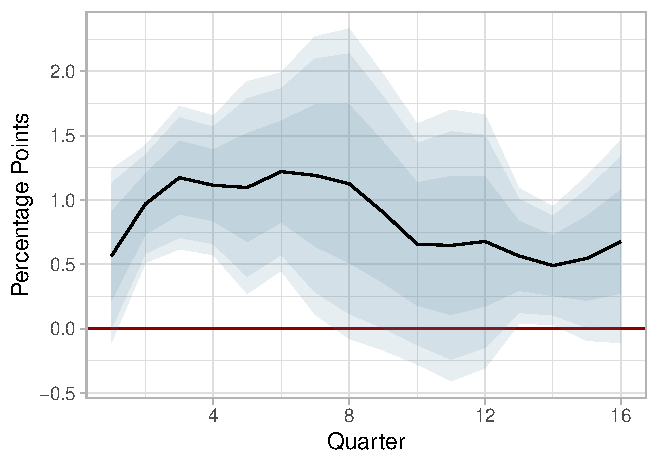
\includegraphics[width=\linewidth]{Average.pdf}
    \end{subfigure}
    \hfill
    \begin{subfigure}[b]{0.49\textwidth}
        \centering
        \caption{Differential Response $(\gamma^h)$}
        \label{fig:DifferentialResponce}
        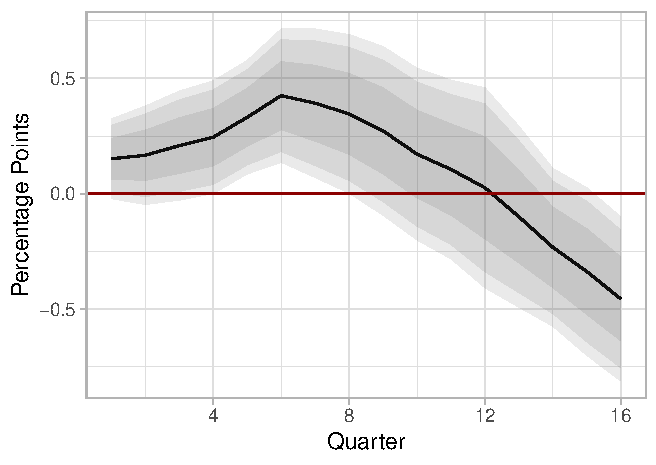
\includegraphics[width=\linewidth]{Differential.pdf}
    \end{subfigure}
        {\begin{flushleft}\scriptsize\textit{Notes}: This figure reports the responses of the $r_t-\rho_t$ to an increase in the Tealbook inflation forecast of 1 p.p. above sample average. The subfigure \ref{fig:AverageResponce} reports the response for the $\mathit{HAWK}$ index equal to the sample average and \ref{fig:DifferentialResponce} is the addition to the response in case there are 2 (out of 12 in total) additional consistent hawks in the FOMC. The shaded areas correspond to 68\%, 90\% and 95\% confidence bands calculated with Newey-West HAC estimator with Andrews-selected truncation parameter.\end{flushleft}}
\end{figure}


\begin{table}[!htb] \centering \scriptsize
    \begin{threeparttable}
    \caption{Size-Persistence Tradeoff} 
    \label{tab:Size-Persistence} 
    \begin{tabular}{@{\extracolsep{10pt}}lcc} 
      \\[-1.8ex]\hline 
      \hline \\[-1.8ex] 
       & \multicolumn{2}{c}{\textit{Dependent variable:}} \\ 
      \cline{2-3} 
      \\[-1.8ex] & \multicolumn{2}{c}{$\log(\mathit{consumption})$} \\ 
      \\[-1.8ex] & (1) & (2)\\ 
      \hline \\[-1.8ex] 
       Size $(R_0)$  & $-$0.687 & $-$0.114 \\ 
        & ($-$1.141, $-$0.125) & ($-$1.495, 1.078)    \\ 
        &[0.011]\{0.997\} & [0.857]\{0.578\}\\ 
        & & \\ 
       Persistence $(\nu)$ & $-$0.100 & 1.223 \\ 
        & ($-$0.694,  0.691)   & ($-$3.598, 4.968)    \\ 
        &[0.746]\{0.673\} & [0.517]\{0.246\}\\ 
        & & \\ 
        $\nu^2$ &  & $-$1.042 \\ 
        &  &  ($-$4.271, 4.336) \\ 
        & &[0.517]\{0.766\} \\ 
        & & \\ 
       $R_0\times \nu$ & 0.765 & $-$1.628 \\ 
        & ($-$0.175,  1.526)    &   ($-$6.095,  4.186)     \\ 
        &[0.0754]\{0.0247\} & [0.522]\{0.759\}\\ 
        & & \\ 
        $R_0\times \nu^2$ &  & 2.435 \\ 
        &  &  ($-$4.017, 6.784) \\ 
        & & [0.340]\{0.145\}\\ 
        & & \\ 
       Constant & 10.608 & 10.224 \\ 
        & (10.06, 10.96) & (9.13, 11.33)    \\ 
        & [0.0]\{0.0\}& [0.0]\{0.0\}\\ 
        & & \\[-1.8ex] 
      \hline \\[-1.8ex] 
      Observations & 198 & 198 \\ 
      R$^{2}$ & 0.338 & 0.343 \\ 
      Adjusted R$^{2}$ & 0.328 & 0.326 \\ 
      Residual Std. Error & 0.245 & 0.245 \\ 
      \hline 
      \hline \\[-1.8ex] 
      \end{tabular} 
    \begin{tablenotes}[flushleft]
    \item[] \scriptsize \textit{Note:} The inference is derived from Block bootstrap with 10,000 replications and block lengths having a geometric distribution with mean $16$. 95\% percentile intervals are in parenthesis. Bootstrap p-values for the two-sided hypothesis ($\mathbb{H}_0:\theta=0$ vs $\mathbb{H}_0:\theta\ne 0$) are in square brackets, p-values for the one-sided hypothesis ($\mathbb{H}_0:\theta=0$ vs $\mathbb{H}_0:\theta>0$) are in curly brackets. 
  \end{tablenotes}
\end{threeparttable}
  \end{table} 


\newpage 

\section{Robustness}
tba


\newpage
\references
\newpage
\appendix
\numberwithin{table}{section}
\numberwithin{figure}{section}

\section{Additional Results}

\begin{table}[!htbp] \centering \scriptsize
    \begin{threeparttable}
    \caption{Response of FOMC to increase in expected inflation} 
    \label{tab:fullcoef} 
  \begin{tabular}{@{\extracolsep{2pt}}lccccccc} 
  \\[-1.8ex]\hline 
  \hline \\[-1.8ex] 
   & \multicolumn{7}{c}{\textit{Dependent variable:}} \\ 
  \cline{2-7} 
  \\[-1.8ex]  & \multicolumn{5}{c}{$r_{t+h}-\rho_{t+h}$}&\multicolumn{2}{c}{First Stage}\\ 
  \\[-1.8ex] & $h=2$&$h=4$ & $h=6$ & $h=8$& $h=10$ &  $\mathit{HAWK}_t-\overline{\mathit{HAWK}}$& ---''--- \\ &&&&&&& $\times\hat\pi$ \\
  \\[-1.8ex] & (1) & (2) & (3) & (4) & (5) & (6)\\ 
  \hline \\[-1.8ex] 
   $\hat\pi_t$ & 0.968$^{***}$ & 1.114$^{***}$ & 1.220$^{***}$ & 1.127$^{*}$ & 0.657 & 0.054 & 0.121 \\ 
   & (0.232) & (0.275) & (0.392) & (0.613) & (0.476) & (0.036) & (0.090) \\ 
    & & & & & & \\ 
    $\left(\mathit{HAWK}_t-\overline{\mathit{HAWK}}\right)$ & $-$2.071 & $-$2.344 & $-$3.686$^{*}$ & $-$1.612 & 0.537 &  &  \\ 
    & (1.314) & (1.753) & (2.214) & (2.657) & (2.791) &  &  \\ 
    & & & & & & \\ 
    $\left(\mathit{HAWK}_t^\mathit{IV}-\overline{\mathit{HAWK}}^\mathit{IV}\right)$ &  &  &  &  &  & 0.738$^{***}$ & 0.803$^{***}$ \\ 
    &  &  &  &  &  & (0.069) & (0.170) \\ 
    & & & & & & & \\ 
    $\hat\pi_t (\mathit{HAWK}_{t}-\overline{\mathit{HAWK}})$ & 0.999 & 1.470$^{**}$ & 2.552$^{***}$ & 2.077$^{**}$ & 1.029 &  &  \\ 
    & (0.653) & (0.748) & (0.885) & (1.054) & (1.140) &  &  \\ 
    & & & & & & \\ 

    $\hat\pi_t \left(\mathit{HAWK}_{t}^\mathit{IV}-\overline{\mathit{HAWK}}^\mathit{IV}\right)$ &  &  &  &  &  & $-$0.101$^{***}$ & 0.148$^{***}$ \\ 
    &  &  &  &  &  & (0.021) & (0.051) \\ 
    & & & & & & \\ 
    & & & & & & \\ 
   $r_{t-1}-\rho_{t-1}$ & 0.779$^{***}$ & 0.747$^{***}$ & 0.252 & 0.310$^{**}$ & $-$0.059 & 0.010 & $-$0.007 \\ 
   & (0.125) & (0.169) & (0.167) & (0.151) & (0.147) & (0.018) & (0.045) \\ 
    & & & & & & \\ 
    $r_{t-2}-\rho_{t-2}$ & $-$0.068 & $-$0.124 & 0.133 & $-$0.003 & 0.015 & $-$0.011 & $-$0.073 \\ 
    & (0.135) & (0.221) & (0.163) & (0.189) & (0.144) & (0.026) & (0.065) \\ 
    & & & & & & \\ 
    $r_{t-3}-\rho_{t-3}$ & 0.244$^{***}$ & $-$0.208 & $-$0.002 & $-$0.345$^{***}$ & $-$0.206$^{**}$ & 0.005 & 0.033 \\ 
    & (0.078) & (0.156) & (0.104) & (0.122) & (0.091) & (0.026) & (0.064) \\ 
    & & & & & & & \\ 
    $r_{t-4}-\rho_{t-4}$ &  $-$0.141 & 0.216 & 0.147 & 0.265 & 0.139 & 0.019 & $-$0.014 \\ 
    & (0.105) & (0.147) & (0.221) & (0.189) & (0.196) & (0.018) & (0.043) \\ 
    & & & & & & \\ 
  $\hat\pi_{t-1}$ & 0.070 & $-$0.156 & 0.002 & $-$0.258 & 0.040 & $-$0.026 & $-$0.133 \\ 
  & (0.371) & (0.204) & (0.351) & (0.249) & (0.216) & (0.053) & (0.129) \\ 
    & & & & & & \\ 
    $\hat\pi_{t-2}$ & $-$0.420$^{*}$ & $-$0.161 & $-$0.369 & $-$0.521 & $-$0.039 & 0.005 & 0.082 \\ 
    & (0.240) & (0.442) & (0.302) & (0.343) & (0.222) & (0.053) & (0.130) \\ 
    & & & & & & \\ 
    $\hat\pi_{t-3}$  & $-$0.323 & $-$0.175 & $-$0.377 & $-$0.074 & $-$0.196 & $-$0.014 & $-$0.046 \\ 
    & (0.431) & (0.215) & (0.276) & (0.164) & (0.255) & (0.053) & (0.130) \\ 
    & & & & & & \\ 
    $\hat\pi_{t-4}$  & $-$0.230 & $-$0.500 & $-$0.550 & 0.024 & 0.478 & 0.040 & 0.337$^{***}$ \\ 
    & (0.327) & (0.361) & (0.551) & (0.486) & (0.411) & (0.038) & (0.094) \\ 
    & & & & & & \\ 
   Constant  & $-$0.185 & $-$0.176 & 0.264 & $-$0.152 & $-$1.160 & $-$0.223$^{***}$ & $-$0.747$^{***}$ \\ 
   & (0.640) & (0.826) & (0.949) & (1.073) & (1.115) & (0.037) & (0.091) \\ 
    & & & & & & \\ 
  \hline \\[-1.8ex] 
  Observations & 192 & 190 & 188 & 186 & 184 & 194 & 194 \\ 
  R$^{2}$ & 0.841 & 0.751 & 0.650 & 0.597 & 0.576 & 0.669 & 0.794 \\ 
  Adjusted R$^{2}$ & 0.832 & 0.735 & 0.628 & 0.571 & 0.549 & 0.649 & 0.781 \\ 
  Residual Std. Error & 1.465 & 1.845 & 2.195 & 2.371 & 2.438 & 0.211 & 0.520 \\ 
  F Statistic &  &  &  &  &  & 33.438& 63.673 \\ 
  Weak Instrument F & 74.0&73.4 &73.2 & 66.2& 58.7\\
    &  81.5 &80.8& 80.7 &78.3 & 74.62\\
  Wu-Hausman & 2.252 & 1.914& 10.0$^{***}$&8.8$^{***}$& 2.0\\
  \hline 
  \hline \\[-1.8ex] 
  \end{tabular} 
  \begin{tablenotes}[flushleft]
\item[] \textit{Note:}  $^{*}$p$<$0.1; $^{**}$p$<$0.05; $^{***}$p$<$0.01
\end{tablenotes}
\end{threeparttable}
  \end{table} 


\section{Data} 

\noindent\textbf{FRED.} I measure consumption expenditure as chained 2017 dollars, seasonally adjusted personal consumption expenditures per capita (A794RX0Q048SBEA) calculated by the U.S. Bureau of Economic Analysis (quarterly). 
To measure $r_t$ I take the minimum of the shadow federal funds rate \citep{WuXia2016} and effective federal funds rate (DFF).

\noindent\textbf{Natural Rate Estimates.}
Natural rate of interest used is estimated by \citet{LW2003} and re-estimated by \citet{HLW2023} to bridge the Covid period.

% \noindent\textbf{Tealbook Inflation Expectations.} 



% \textbf{}


% \textbf{Consumption}

% \section{Summary statistics}
% \label{sec:SummaryStatistics}
% \begin{table}[!h]
%     \begin{threeparttable}[t]
%     \caption{Summary Statistics} 
%     \label{tab:Summary} 
%     \footnotesize
%     \begin{tabular}{@{\extracolsep{5pt}}lccccccc} 
%         \\[-1.8ex]\hline 
%         \hline \\[-1.8ex] 
%         Statistic & \multicolumn{1}{c}{N} & \multicolumn{1}{c}{Mean} & \multicolumn{1}{c}{St. Dev.} & \multicolumn{1}{c}{Min} & \multicolumn{1}{c}{Pctl(25)} & \multicolumn{1}{c}{Pctl(75)} & \multicolumn{1}{c}{Max} \\ 
%         \hline \\[-1.8ex] 
%         Identified Monetary Shocks\tnote{a} & 348 & $-$0.003 & 0.086 & $-$0 & 0 & 0 & 1 \\
%         $\hat{R}$ & 514 & $-$1.273 & 0.929 & $-$3 & $-$2.2 & $-$0.6 & 0 \\ 
%         Consumption & 171 & 101.202 & 6.622 & 89.544 & 95.518 & 106.610 & 113.121 \\ 
%         Inflation\tnote{b} & 514 & 2.924 & 1.905 & 1.119 & 1.628 & 3.737 & 8.545 \\ 
%         \\
%         \multicolumn{8}{l}{\textit{Treasuty Rates}}\\
%         DGS1 & 514 & 4.959 & 3.836 & 0.097 & 1.545 & 7.313 & 16.719 \\ 
%         DGS2 & 514 & 5.254 & 3.793 & 0.211 & 1.774 & 7.751 & 16.458 \\ 
%         DGS5 & 514 & 5.749 & 3.530 & 0.620 & 2.687 & 8.021 & 15.930 \\ 
%         DGS7 & 514 & 6.001 & 3.403 & 0.984 & 3.072 & 8.219 & 15.648 \\ 
%         DGS10 & 514 & 6.182 & 3.271 & 1.504 & 3.564 & 8.282 & 15.324 \\ 
%         DGS20 & 514 & 6.536 & 3.063 & 1.822 & 4.343 & 8.377 & 15.130 \\ 
%         DGS30 & 514 & 6.562 & 2.956 & 2.119 & 4.396 & 8.448 & 14.684 \\ 
%         \\
%         \multicolumn{8}{l}{\textit{Natural(neutral) Rate estimation by }}\\
%         Neutral Rate& 74 & 1.234 & 0.945 & 0.029 & 0.469 & 2.346 & 2.967 \\ 
%         Neutral Rate monthly & 171 & 0.855 & 0.681 & 0.029 & 0.420 & 0.854 & 2.520 \\ 
%         \\

%         Deviation\tnote{b} & 171 & 0.666 & 0.953 & $-$0.721 & $-$0.081 & 1.141 & 2.819\\
%         Consumption Elasticity & 348 & $-$0.012 & 0.051 & $-$0.214 & $-$0.028 & 0.012 & 0.073 \\ 


%         \hline \\[-1.8ex] 
%         \end{tabular} 
%         \begin{tablenotes}[flushleft]\scriptsize
%             \item Some of the variables start from 1977-04-01. We estimate main relations above starting from 1990-01-01 to keep the monetary well-identified.
%             \item[a] \cite{BRW2021} style identified monetary shocks.
%          \item[b] We use smoothed PCEPILFE monthly change to estimate inflation
%          \item[b] $R_{DSG2}-$
%         \end{tablenotes}
%     \end{threeparttable}
%   \end{table} 


% \begin{figure}[h!]\centering
%     \begin{minipage}{\textwidth}
%     \caption{Deviation of DGS2 interest rate from Natural rate of interest and its components} 
%     \label{fig:Deviation}
%     % \includegraphics[width=\linewidth]{deviation.pdf}
%     {\raggedleft\scriptsize Natural rate of interest estimated by {\protect\citet{HLW2017}}.  US recessions are shaded.} 
%     \end{minipage}
% \end{figure}


% \begin{figure}[!htbp]\centering
%     \begin{minipage}{0.6\textwidth}
%     \caption{Hausman test of sum of monetary shocks as IV P-statistic}
%     \label{fig:Hausman}
%     {\raggedleft\scriptsize This figure provides Hausman test p-values}
%     \end{minipage}
% \end{figure}

% \begin{figure}[!htbp]\centering
%     \begin{minipage}{\textwidth}
%     \caption{ARMA$(p,q)$ contemporaneously estimated in a window }
%     \vspace{2ex}
%     \begin{minipage}{\textwidth}
% \end{minipage}
%     \\
%     \begin{minipage}{\textwidth}
%     % \includegraphics[width=0.32\textwidth]{ar4Plot.pdf}
%     % \includegraphics[width=0.32\textwidth]{ma1Plot.pdf}
%     % \includegraphics[width=0.32\textwidth]{ma2Plot.pdf}
% \end{minipage}
% \begin{flushleft}\scriptsize
%     This figure show the decomposition of the unrestricted estimated ARMA$(p,q)$ model over \citet{BRW2021} identified monetary shock. 
% \end{flushleft}
%     \end{minipage}
% \end{figure}







\end{document}